\chapter{Implementation Details}
\label{chap:implementation_detail}
\section{Introduction}
\label{sec:intro}

% Discuss about PySPH, What PySPH provides. what all is implemented, what kind
% of algorithms are implemented,
In the current chapter, we detail the algorithms implemented in the current work
in order to handle the collision among bodies and discuss the implementation
details of the sub-stepping algorithm while handling different materials in a
simulation. We discuss the implementation details and outline the implementation
of the algorithms proposed in earlier chapters and the upcoming ones. The
current work is implemented in an open-source framework, PySPH
\parencite{pysph2020}. In PySPH, particle arrays are initiated using a structure of
arrays formulation, with each index corresponding to a particle. Equations
compute accelerations on the particles using these particle arrays. PySPH is
primarily written to model SPH schemes. However, it can be used to implement
other meshless techniques as well. PySPH has several SPH methods implemented,
such as, WCSPH, TVF, and Godunov SPH, to note a few among others. The
documentation at \url{https://pysph.readthedocs.io} covers details on how to
implement new SPH algorithms in PySPH in some detail. We assume the reader to
have some familiarity with PySPH and one may safely skip the chapter if one
is not interested in the details.


% Write the difficulty of implementing contact algorithm in PySPH (discuss
% linked list). No documentation regarding the multiphase or we write here.
We implement the discretized equations of \cref{chap:ctvf} following the PySPH
documentation. In order to implement the contact force formulation developed in
\cref{chap:csph}, we need to track the pairwise quantities to evolve the
tangential force with time. However, the PySPH documentation does not describe
how to implement such algorithms. SPH is used to model fluid and structural
dynamics through the current work. Collision among elastic solids is handled
with a contact force as demonstrated in \cref{chap:csph}. The discretized
governing equations of the fluid and the solid do not need to track the
particles which are in contact. However, to implement contact interaction for
DEM we need to keep track of the tangential displacement per particle. It is not
straightforward to implement the per-particle pairwise interaction with the
philosophy of PySPH. We show how this can be done in this chapter.

When simulating different materials, they often require different timesteps. A
sub-stepping algorithm is suitable, where a material with a larger timestep is
updated first with a larger timestep, and a material with a smaller timestep is
updated with a smaller timestep. Substepping is efficient as it reduces
computations for the material with a higher timestep. The documentation at
\url{https://pysph.readthedocs.io} doesn't provide clear details on how to
implement this algorithm. However, PySPH provides tools to implement this. We
consider a problem involving fluid and solids to demonstrate a sub-stepping
algorithm. The implemented sub-stepping algorithm is used in \cref{chap:fsi}.
Minimal code snippets are provided covering the basic outline of the algorithm.


\FloatBarrier%
\section{Contact Force Modeling with a Few Number of Bodies}
\label{sec:tracking-few-bodies}
In this section, we compute the contact force on a particle due to the
interaction with three other bodies composed of particles. As a representative
example, we consider the collision of four bodies. \Cref{fig:id:four_bodies_contact}
shows the schematic of the bodies at three different instants. This example is
utilized to describe the contact force algorithm implemented in \cref{chap:csph}
where elastic solids are colliding.
\begin{figure}[!htpb]
  \centering
  \begin{subfigure}{0.32\textwidth}
    \centering
    \includegraphics[width=1.0\textwidth]{images/implementation_detail/images/few_bodies/four_bodies_initial}
    \subcaption{Bodies at time $t=0$ seconds.}%\label{fig:rings:ipst-nu-0.47-0}
  \end{subfigure}
  \begin{subfigure}{0.32\textwidth}
    \centering
    \includegraphics[width=1.0\textwidth]{images/implementation_detail/images/few_bodies/four_bodies_interact}
    \subcaption{Bodies at time $t_1$ seconds.}%\label{fig:rings:ipst-nu-0.47-0}
  \end{subfigure}
  \begin{subfigure}{0.32\textwidth}
    \centering
    \includegraphics[width=1.0\textwidth]{images/implementation_detail/images/few_bodies/four_bodies_final}
    \subcaption{Bodies at time $t_2$ seconds.}%\label{fig:rings:ipst-nu-0.47-0}
  \end{subfigure}
  \caption{Snapshots of four bodies colliding.}
\label{fig:id:four_bodies_contact}
\end{figure}


To demonstrate the algorithm, we consider the computation of contact force on
particles of the body $1$. A particle of the body can be in contact with the
other three bodies. To compute the contact force on particle $a$ of the body $x$
due to the interaction with body $y$, where $a,$ $x$, and $y$ are natural
numbers, we need to compute the overlap of particle $a$ with body $y$ at every
time instant. The contact overlap evolves with time until the body $y$ stays in
contact with particle $a$. To evolve this pairwise quantity, we need to keep
track of the overlap amount with the bodies. One way to do this is as follows,
as soon as the body comes into contact, we insert the new element in a linked
list data structure to track the overlap with this body, and the value of this
is retrieved and updated until the body stays in contact with the particle.
However, PySPH does not allow one to use a linked list data structures. Here, we
propose an algorithm where we can track these pairwise contact quantities using
one-dimensional arrays. A unique \texttt{body\_id} is assigned to each particle. In the
current case, all particles belonging to the body $0$ in
\cref{fig:id:four_bodies_contact} have their \texttt{body\_id} set to $0$. This
property is used to index the pairwise contact property of a particle with other
bodies. To demonstrate the algorithm, we consider the computation of contact
force on particles of the body $1$, such that $x=1$ and $y$ corresponds to
$0, 2, 3$. We create an array of length $M \times total\_no\_bodies$. Here, $M$
is the total no of particles of the body $1$. This array is used to save the
pairwise quantities, such as contact overlap. Each particle is assigned a chunk,
in the current case, a chunk of size $4$, as the total number of bodies in the
simulation is $4$. This is depicted in \cref{fig:stride_index_trace}, which
shows the state of the arrays at the time of initiation. Since at time $t=0$, no
bodies are overlapping, we initialize the pairwise overlap quantity to $0$. From
\cref{fig:stride_index_trace}, we can see that each particle is assigned a chunk
of size $4$. Specially, \cref{fig:stride_index_trace} shows the array values for
particles with index $0, k$ and $M-1$. Since the number of bodies is small, we
assign a constant index for each possible pair. This can be seen in
\cref{fig:stride_index_trace}, as particle id of $0, k$ and $M-1$, has a
corresponding array space to track the pairwise quantity, such as overlap, with
four bodies in the simulation. However, in the current case, we assume that a
particle could not be in contact with the body it belongs to. So the
corresponding array element entry would remain $0$ or to the initialized value
the throughout the simulation.
\begin{figure}[!htpb]
  \centering
  \footnotesize
  \begin{tikzpicture}
    \matrix (m) [matrix of nodes,
    nodes={draw, minimum size=10mm,anchor=center},
    nodes in empty cells, minimum height = 1cm,
    row 1/.style={nodes={draw=none}},]
    {
      particle id: & 0 & 0 & 0 & 0 &          & k  & k    & k    & k    &          & M-1  & M-1  & M-1  & M-1 \\
      $body\_id$:  & 0 & 1 & 2 & 3 &          & 0  & 1    & 2    & 3    &          & 0    & 1    & 2    & 3 \\
      overlap:     & 0 & 0 & 0 & 0 & $\cdots$ & 0  & 0    & 0    & 0    & $\cdots$ & 0    & 0    & 0    & 0\\
      Index  :     & 0 & 1 & 2 & 3 & $\cdots$ & 4k & 4k+1 & 4k+2 & 4k+3 & $\cdots$ & 4M-4 & 4M-3 & 4M-2 & 4M-1\\
    };
  \end{tikzpicture}
  \caption{An array to track the pairwise quantities. A stride of length $4$ is
    assigned to each particle to track the pairwise quantity.}
\label{fig:stride_index_trace}
\end{figure}

At an intermediate time $t_1$, let us assume that a particle with an index $k$ of body
$1$ is in contact with body $2$ and particle with index $l$ with body $3$ as seen in
\cref{fig:id:four_bodies_contact}. The updated overlap amount of particles $k$
and $l$ is given in \cref{fig:id:k_f_overlap_t_1},
\begin{figure}[!htpb]
  \centering
  \footnotesize
  \begin{tikzpicture}
    \matrix (m) [matrix of nodes,
    nodes={draw, minimum size=10mm,anchor=center},
    nodes in empty cells, minimum height = 1cm,
    row 1/.style={nodes={draw=none}},]
    {
      particle id: & & k & k & k & k & & l & l & l & l &  \\
      $body\_id$:  & & 0 & 1 & 2 & 3 & & 0 & 1 & 2 & 3 &  \\
      Index & $\cdots$ & 4k & 4k+1 & 4k+2 & 4k+3 & $\cdots$ & 4l & 4l+1 & 4l+2 & 4l+3 & $\cdots$ \\
      Overlap & $\cdots$ & 0 & 0 & $\psi_1$ & 0 & $\cdots$ & 0 & 0 & 0 & $\psi_2$ & $\cdots$ \\
    };
  \end{tikzpicture}
  \caption{Updated overlap amount of particles $k$ and $l$.}
\label{fig:id:k_f_overlap_t_1}
\end{figure}
where $\psi$ in the figure is a real number. Since particle $k$ is in contact
with body id $2$, we can see from \cref{fig:id:k_f_overlap_t_1} that the overlap
amount of particle $k$ with body id $2$ is saved as $\psi_1$. This overlap
amount is saved at its fixed array index of $4k+2$. Since particle $l$ is in
contact with body id $3$, we save the overlap with body $3$ at $4l+3$ index.
Similarly, let us assume a particle with an index $q$ is in contact with the
body $2$ and $3$. The pairwise array belonging to the particle $q$ is shown in
\cref{fig:id:overlap_of_q_at_t_1}. From \cref{fig:id:overlap_of_q_at_t_1}, we
can see that the pairwise overlap quantity of particle $q$ with bodies $2$ and
$3$ are saved at the indices of $4q+2$ and $4q+3$, respectively.
\begin{figure}[!htpb]
  \centering
  \footnotesize
  \begin{tikzpicture}
    \matrix (m) [matrix of nodes,
    nodes={draw, minimum size=12mm,anchor=center},
    nodes in empty cells, minimum height = 1cm,
    row 1/.style={nodes={draw=none}},]
    {
      Body Id: & & 0 & 1 & 2 & 3 & & \\
      Index & $\cdots$ & 4q & 4q+1 & 4q+2 & 4q+3 & $\cdots$ \\
      Overlap & $\cdots$ & 0 & 0 & $\psi_1$ & $\psi_2$ & $\cdots$ \\
    };
  \end{tikzpicture}
  \caption{Overlap amount of particle $q$ when in contact with bodies $2$ and $3$.}
  \label{fig:id:overlap_of_q_at_t_1}
\end{figure}

At the time ($t_3$), let the particle $l$ lose its collision with body $3$,
while particle $k$ is still in contact with body $2$. The updated overlap array
for this configuration is shown in \cref{fig:id:overlap_of_k_f_at_t_2}. From
\cref{fig:id:overlap_of_k_f_at_t_2}, we can see that we have updated the
pairwise tracking quantity, overlap, we make the overlap array value at index
$4l+3$ zero, as the particle $l$ lost contact with body $3$. However, we keep
the overlap value of particle $k$ with body $2$ since it didn't lose contact
with it.

\begin{figure}[!htpb]
  \centering
  \footnotesize
  \begin{tikzpicture}
    \matrix (m) [matrix of nodes,
    nodes={draw, minimum size=12mm,anchor=center},
    nodes in empty cells, minimum height = 1cm,
    row 1/.style={nodes={draw=none}},]
    {
      Body Id: & & 0 & 1 & 2 & 3 & &  0 & 1 & 2 & 3 & & \\
      Index & $\cdots$ & 4k & 4k+1 & 4k+2 & 4k+3 & $\cdots$ & 4l & 4l+1 & 4l+2 & 4l+3 & $\cdots$ \\
      Overlap & $\cdots$ & 0 & 0 & $\psi_1$ & 0 & $\cdots$ & 0 & 0 & 0 & 0 & $\cdots$ \\
    };
  \end{tikzpicture}
  \caption{Overlap array of body $1$, showing the specific indices of
    particles $k$ and $l$ at time $t_2$.}
\label{fig:id:overlap_of_k_f_at_t_2}
\end{figure}
While letting particle $q$ lose its contact with bodies $2$ and $3$ and come
into contact with body $0$. In this case, the updated overlap array for the
indices belonging to the particle $q$ is given in
\cref{fig:id:overlap_of_q_at_t_2}. Similar to particle $k$ and $l$, we update
the pairwise tracking quantity, however, we save the overlap amount of particle
$q$ with body $0$ and make overlap amounts to zero for the indices of $4q+2$ and
$4q+3$.
\begin{figure}[!htpb]
  \centering
  \footnotesize
  \begin{tikzpicture}
    \matrix (m) [matrix of nodes,
    nodes={draw, minimum size=12mm,anchor=center},
    nodes in empty cells, minimum height = 1cm,
    row 1/.style={nodes={draw=none}},]
    {
      Body Id: & & 0 & 1 & 2 & 3 & & \\
      Index & $\cdots$ & 4q & 4q+1 & 4q+2 & 4q+3 & $\cdots$ \\
      Overlap & $\cdots$ & $\psi_1$ & 0 & 0 & 0 & $\cdots$ \\
    };
  \end{tikzpicture}
  \caption{Overlap array of body $1$, showing the index of
    particle $q$ at time $t_2$.}
\label{fig:id:overlap_of_q_at_t_2}
\end{figure}
In the next section we look at the code to implement this algorithm in
PySPH.

\FloatBarrier%
\subsection{Implementation in PySPH}
We implement the above algorithm in PySPH using the following code. We first
create a particle array with the required properties. A sample code segment
describing the creation of a particle array is given as
\lstset{caption={Code segment for the creation of a particle array.}} \lstset{basicstyle=\footnotesize\ttfamily}
\begin{lstlisting}[label={contact:equations},frame=lines,language=Python,upquote=True]
body_2 = get_particle_array(x=[0., 1., 2., 3.],
                            y=[0., 0., 0., 0.],
                            # ... Code redacted ...
                            name="body")
\end{lstlisting}

To implement the pairwise tracking algorithm, we add an additional property with
a stride. In our case, a particle can contact four bodies at a given time. A
property of stride length $4$ is added to the particle array as
\lstset{caption={Code segment to add a stride property to an existing particle
    array.}} \lstset{basicstyle=\footnotesize\ttfamily}
\begin{lstlisting}[label={contact:equations},frame=lines,language=Python,upquote=True]
body_2.add_property(name='overlap', stride=4)
\end{lstlisting}
The pairwise interactions are computed with the following code
\lstset{caption={Code snippet to handle tracking of pairwise interactions with a few number of bodies.}} \lstset{basicstyle=\footnotesize\ttfamily}
\begin{lstlisting}[label={contact:equations},frame=lines,language=Python,upquote=True]
class ComputeContactForce(Equation):
    def initialize(self, d_idx, d_overlap, d_total_no_bodies, dt, t):
        i, t1, t2 = declare('int', 3)

        t1 = d_total_no_bodies[0] * d_idx

        for i in range(d_total_no_bodies[0]):
            t2 = t1 + i
            d_overlap[t2] = 0.

    def loop(self, d_idx, d_total_no_bodies, s_idx,
            s_body_id, dt, RIJ):
        t1, t2 = declare('int', 2)

        t1 = d_total_no_bodies[0] * d_idx
        t2 = t1 + s_body_id[s_idx]

        d_overlap[t2] += RIJ
        # ... Code redacted ...
\end{lstlisting}
Here, \textit{d\_total\_no\_bodies} is the total number of bodies in a given
case. In the above code listing, in order to compute the overlap of the
particles on a given body with the other bodies, we first initialize the
pairwise quantity, overlap, to zero. \texttt{initialize} method depicts the
initialization of overlap to zero. In \texttt{loop} method, we compute the pairwise
overlap of the particle when colliding with the bodies. We compute the forces on
the bodies using the above equation using the \texttt{Group} function in PySPH
\texttt{Application} class routine as, 2.1 $2.1$
\lstset{caption={Code segment to compute the forces on the bodies.}} \lstset{basicstyle=\footnotesize\ttfamily}
\begin{lstlisting}[label={contact:equations},frame=lines,language=Python,upquote=True]
  Group(equations=[
      ComputeContactForce(dest='body_0', sources=[
          'body_1', 'body_2', 'body_3']),
      ComputeContactForce(dest='body_1', sources=[
          'body_1', 'body_2', 'body_3']),
      ComputeContactForce(dest='body_2', sources=[
          'body_1', 'body_2', 'body_3']),
      ComputeContactForce(dest='body_3', sources=[
          'body_0', 'body_1', 'body_2'])
    ])
\end{lstlisting}
We execute the equation of computation of the contact force of each body due to the
\texttt{sources}. Four equations are used to compute the forces on four bodies due to
the interaction with the other three bodies.


\FloatBarrier%
\section{Contact Force Modeling with a Large Number of Particles}
\label{sec:tracking-many-bodies}
In the previous section, we used a strided array with a fixed index per
interaction to handle the tracking of pairwise interactions while computing the
contact force on a particle due to the interaction with other bodies. However, a
fixed index per interaction is not favorable when dealing with simulations
involving a large number of bodies or particles. This is because, a very large
stride is wasteful in terms of memory. For cases with a large number of bodies,
we propose an algorithm where dynamic addition and removal of contacts are
involved. Further, this algorithm is feasible in cases when the particle at a
given time will not have more than a fixed number of contacts to track. In the
current section, we demonstrate the dynamic contact handling algorithm. We
consider two cases, one where all the particles belong to the same particle
array and another case where particles belonging to two different particle
arrays interact with each other and among themselves.

\subsection{Single Particle Array}
\begin{figure}[!htpb]
  \centering
  \includegraphics[width=0.3\textwidth]{images/implementation_detail/images/many_bodies/many_bodies_t_0}
  \caption{Particles with finite radius at time $t=0$.}
\label{fig:id:15_particle_t_0}
\end{figure}

To demonstrate the dynamic tracking algorithm, we consider the interaction of
$15$ particles as shown in \cref{fig:id:15_particle_t_0}. We assume, at a given
time, no particle can have more than $3$ contacts. We demonstrate the algorithm
when the particles are initiated in a single particle array, such that no two
particles have the same index. Since, with a large number of bodies involved, we
do not have a prefixed index for the pairwise interaction, we additionally need
to save the index of the contacting particle in addition to the pairwise contact
properties. \Cref{fig:many_bodies_initialize_overlap_t_0}, shows the additional
property, \texttt{contact\_id}, added to the particle array to track the indices which a
given particle of index $k$ is in contact with. The contact indices are
initialized to $-1$ and other pairwise interaction properties are initialized to
$0$ similar to the previous algorithm.
\begin{figure}[!htpb]
  \centering
  \footnotesize
  \begin{tikzpicture}
    \matrix (m) [matrix of nodes,
    nodes={draw, minimum size=10mm,anchor=center},
    nodes in empty cells, minimum height = 1cm,
    row 1/.style={nodes={draw=none}},]
    {
      Particle id: & 0 & 0 & 0 & & k & k & k & & 14 & 14  & 14 \\
      Contact Id: & -1 & -1 & -1 &  & -1 & -1 & -1 & & -1 & -1 & -1  \\
      Index: & 0 & 1 & 2 & $\cdots$ & 4k & 4k+1 & 4k+2 & $\cdots$ & 42 & 43 & 44 \\
      Overlap: & 0 & 0 & 0 & $\cdots$ & 0 & 0 & 0 & $\cdots$ & 0 & 0 & 0 \\
    };
  \end{tikzpicture}
  \caption{Values of strided array properties to handle the tracking of many bodies at time $t=0$.}
\label{fig:many_bodies_initialize_overlap_t_0}
\end{figure}

Code fragment of adding the new stride properties is given as
\lstset{caption={Code fragment to add the property required to track dynamics contacts.}} \lstset{basicstyle=\footnotesize\ttfamily}
\begin{lstlisting}[label={contact:equations},frame=lines,language=Python,upquote=True]
  pa.add_property('contact_id', stride=3, type="int")
  pa.contact_id[:] = -1
  pa.add_property(name='overlap', stride=3)
\end{lstlisting}

\begin{figure}[!htpb]
  \centering
  \includegraphics[width=0.3\textwidth]{images/implementation_detail/images/many_bodies/many_bodies_t_1}
  \caption{Configuration of particles at an intermediate time $t_1$.}
\label{fig:id:15_particle_t_1}
\end{figure}
%
The configuration of particles at an intermediate time $t_1$ are shown in
\cref{fig:id:15_particle_t_1}. Particles marked in red are contacts of $1$, $8$,
and $11$ particles. From \cref{fig:id:15_particle_t_1}, we can see that
particle with index $1$ is in contact with $0, 6, 7$ particles and a particle
with index $8$ with $5$ and $9$. Let us assume the contacts are formed for the
first time. \Cref{fig:many_bodies_initialize_overlap_1_8_11_t_1} shows the
updated overlap array of the contact indices, including the overlap for the
particles with index $1, 8$, and $11$.
\begin{figure}[!htpb]
  \centering
  \footnotesize
  \begin{tikzpicture}
    \matrix (m) [matrix of nodes,
    nodes={draw, minimum size=10mm,anchor=center},
    nodes in empty cells, minimum height = 1cm,
    row 1/.style={nodes={draw=none}},]
    {
      Contact Id: & $\cdots$ & 0 & 6 & 7 &  & 5 & 9 & -1 & & 14 & -1 & -1 & & \\
      Index & $\cdots$ & 3 & 4 & 5 & $\cdots$ & 24 & 25 & 26 & $\cdots$ & 33 & 34 & 35 & $\cdots$\\
      Overlap  &$\cdots$ & $\psi_1$ & $\psi_2$ & $\psi_3$ & $\cdots$ & $\psi_4$ & $\psi_5$ & 0 & $\cdots$ & $\psi_6$ & 0 & 0 & $\cdots$ \\
    };
  \end{tikzpicture}
  \caption{Updated Contact Id and Overlap array at an intermediate time $t_1$.}
\label{fig:many_bodies_initialize_overlap_1_8_11_t_1}
\end{figure}

Dynamic pairwise contact tracking is handled in two parts. The first part is to
update the tracking array by removing the indices which are no more in contact.
As a second step, we add new contacts. We use two equations to implement it in
PySPH. One equation is used to add new contacts and update the values of the
existing contacts, while the second equation can be used to remove the
indices that are no more in contact. We outline the code to add new contacts and
update the existing ones in the following code snippet.
\lstset{caption={Code snippet to add new contact and update existing contact properties in dynamic
    pairwise tracking algorithm.}} \lstset{basicstyle=\footnotesize\ttfamily}
\begin{lstlisting}[label={code:add_contacts_many},frame=lines,language=Python,upquote=True]
class AddParticlesInContact(Equation):
    def loop(self, d_idx, d_m, d_contact_id, d_overlap, d_total_contacts,
             d_max_contacts_limit, RIJ, d_rad, s_idx, s_rad):
        p, q1, tot_ctcs, j, found_at, found = declare('int', 6)
        overlap = -1.

        # check the particles are not on top of each other.
        if RIJ > 1e-12:
            overlap = d_rad[d_idx] + s_rad[s_idx] - RIJ

        # ---------- force computation starts ------------
        # if particles are overlapping
        if overlap > 0:
            # total number of contacts of particle i in destination
            tot_ctcs = d_total_contacts[d_idx]

            # d_idx has a range of tracking indices with sources
            # starting index is p
            p = d_idx * d_max_contacts_limit[0]
            # ending index is q -1
            q1 = p + tot_ctcs

            # check if the particle is in the tracking list
            # if so, then save the location at found_at
            found = 0
            for j in range(p, q1):
                if s_idx == d_contact_id[j]:
                    found_at = j
                    found = 1
                    break
            # if the particle is not been tracked then assign an
            # index in tracking history.
            if found == 0:
                found_at = q1
                d_contact_id[found_at] = s_idx
                d_total_contacts[d_idx] += 1

            # implies we are tracking the particle
            else:
                # Save the pair wise quantity at found_at
                d_overlap[found_at] = overlap
\end{lstlisting}


\begin{figure}[!htpb]
  \centering
  \includegraphics[width=0.3\textwidth]{images/implementation_detail/images/many_bodies/many_bodies_t_2}
  \caption{configuration of particles at time $t_2$.}
\label{fig:id:15_particle_t_2}
\end{figure}

\Cref{fig:id:15_particle_t_2} shows the particles positions at time $t_2$. From
\cref{fig:id:15_particle_t_2}, we can see that a few particles lose contacts,
and a few gain new contacts. We will add the new particles to the tracking array
using the above code. However, after every time step, first we need to update
the tracking array by removing the indices that are no more in contact.
\Cref{fig:many_bodies_initialize_overlap_1_8_11_t_2} shows the updated contact
indices array and the overlapping array at time $t_2$.
\begin{figure}[!htpb]
  \centering
  \begin{tikzpicture}
    \matrix (m) [matrix of nodes,
    nodes={draw, minimum size=10mm,anchor=center},
    nodes in empty cells, minimum height = 1cm,
    row 1/.style={nodes={draw=none}},]
    {
      Contact Id: & $\cdots$ & 6 & 7 & -1 &  & 13 & -1 & -1 & & 12 & -1 & -1 & & \\
      Index & $\cdots$ & 3 & 4 & 5 & $\cdots$ & 24 & 25 & 26 & $\cdots$ & 33 & 34 & 35 & $\cdots$\\
      Overlap  &$\cdots$ & $\psi_1$ & $\psi_2$ & 0 & $\cdots$ & $\psi_3$ & 0 & 0 & $\cdots$ & $\psi_4$ & 0 & 0 & $\cdots$ \\
    };
  \end{tikzpicture}
  \caption{Updated Contact Id and Overlap array at an intermediate time $t_2$}
\label{fig:many_bodies_initialize_overlap_1_8_11_t_2}
\end{figure}

The following code snippet is used to remove the contacts that are no more in
contact with the particle.
\lstset{caption={Code snippet to remove lost contacts in dynamic pairwise tracking algorithm.}} \lstset{basicstyle=\footnotesize\ttfamily}
\begin{lstlisting}[label={contact:equations},frame=lines,language=Python,upquote=True]
class RemoveParticlesNotInContact(Equation):
    def initialize_pair(self, d_idx, d_x, d_y, d_z, d_rad,
                        d_total_contacts, d_contact_id,
                        d_max_contacts_limit, d_overlap,
                        s_rad):
        # Declare variable: Code redacted

        idx_total_ctcs = d_total_contacts[d_idx]
        # particle idx contacts has range of indices
        # and the first index would be
        p = d_idx * d_max_contacts_limit[0]
        last_idx_tmp = p + idx_total_ctcs - 1
        k = p
        count = 0

        # loop over all the contacts of particle d_idx
        while count < idx_total_ctcs:
            # The index of the particle with which
            # d_idx in contact is
            sidx = d_contact_id[k]

            if sidx == -1:
                break
            else:
                xij[0] = d_x[d_idx] - s_x[sidx]
                xij[1] = d_y[d_idx] - s_y[sidx]
                xij[2] = d_z[d_idx] - s_z[sidx]
                rij = sqrt(xij[0] * xij[0] + xij[1] * xij[1] +
                           xij[2] * xij[2])

                overlap = d_rad_s[d_idx] + s_rad_s[sidx] - rij

                if overlap <= 0.:
                    # if the swap index is the current index then
                    # simply make it to null contact.
                    if k == last_idx_tmp:
                        d_contact_id[k] = -1
                        d_overlap[k] = 0.
                    else:
                        # swap the current tracking index with the final
                        # contact index
                        d_contact_id[k] = d_contact_id[last_idx_tmp]
                        d_contact_id[last_idx_tmp] = -1

                        # swap tangential x displacement
                        d_overlap[k] = d_overlap[last_idx_tmp]
                        d_overlap[last_idx_tmp] = 0.

                        # decrease the last_idx_tmp, since we swapped it to
                        # -1
                        last_idx_tmp -= 1

                    # decrement the total contacts of the particle
                    d_total_contacts[d_idx] -= 1
                else:
                    k = k + 1
                count += 1
\end{lstlisting}

The above equations are used in the \texttt{create\_equations} method of \texttt{Application}
class of PySPH to execute in execution loop using the following code.
\lstset{caption={An equation execution order to handle the pairwise tracking algorithm in PySPH.}} \lstset{basicstyle=\footnotesize\ttfamily}
\begin{lstlisting}[label={contact:equations},frame=lines,language=Python,upquote=True]
  Group(equations=[
      RemoveParticlesNotInContact(dest='grains',
      sources=['grains'])
    ]),
  Group(equations=[
      AddParticlesInContact(dest='grains', sources=['grains'])
    ]),
\end{lstlisting}


\FloatBarrier%
\subsection{Dealing with Multiple Particle Arrays}
Let us consider a case where particles of two different particle arrays
interact with each other. A schematic is shown in \cref{fig:mb:2_pa}. Here,
we consider each particle array to have $15$ particles, as shown in
\cref{fig:mb:2_pa}.
\begin{figure}[!htpb]
  \centering
  \includegraphics[width=0.7\textwidth]{images/implementation_detail/images/many_bodies/many_bodies_two_pa_t_0}
  \caption{}
\label{fig:mb:2_pa}
\end{figure}
Let's name particle array $1$ as \texttt{grains\_1} and particle array $2$ as
\texttt{grains\_2}. As described in the previous section, in PySPH, to compute
the interaction, we use the following code snippet.
\lstset{caption={Code snipped to compute contact force on particle arrays.}}
\lstset{basicstyle=\footnotesize\ttfamily}
\begin{lstlisting}[label={contact:equations},frame=lines,language=Python,upquote=True]
  Group(equations=[
      RemoveParticlesNotInContact(dest='grains_1',
          sources=['grains_1', 'grains_2'])
      RemoveParticlesNotInContact(dest='grains_2',
          sources=['grains_1', 'grains_2'])
    ]),
  Group(equations=[
      AddParticlesInContact(dest='grains_1',
          sources=['grains_1', 'grains_2'])
      AddParticlesInContact(dest='grains_2',
          sources=['grains_1', 'grains_2'])
    ]),
\end{lstlisting}


Let us consider the computation of contact force on particles belonging to
particle array 1. From the previous algorithm, we initialize the
\texttt{contact\_id} and \texttt{overlap} arrays to particle array $1$ as shown
in \cref{fig:mb-2-pa-prev-algo}.
\begin{figure}[!htpb]
  \centering
  \begin{tikzpicture}
    \matrix (m) [matrix of nodes,
    nodes={draw, minimum size=12mm,anchor=center},
    nodes in empty cells, minimum height = 1cm,
    row 1/.style={nodes={draw=none}},]
    {
      Contact Id: & -1 & -1 & -1 &  & -1 & -1 & -1 & & -1 & -1 & -1  \\
      Index & 0 & 1 & 2 & $\cdots$ & 4k & 4k+1 & 4k+2 & $\cdots$ & 42 & 43 & 44 \\
      Overlap & 0 & 0 & 0 & $\cdots$ & 0 & 0 & 0 & $\cdots$ & 0 & 0 & 0 \\
    };
  \end{tikzpicture}
  \caption{Contact Id and Overlap array for particle array 1.}
\label{fig:mb-2-pa-prev-algo}
\end{figure}

\Cref{fig:mb-2-pa-t-2} shows the particle arrays' particles
interacting with each other. From \cref{fig:mb-2-pa-t-2}, we can see particles
of both arrays interact with each other. \Cref{fig:zoomed-8-id} depicts
contacts of particle with index $8$. The contact array and the pairwise overlap
of a particle with index $8$ are shown in \cref{fig:id-8-mb-array}. From
\cref{fig:id-8-mb-array,fig:zoomed-8-id}, we can see that the particle with
index $8$ is in contact with a particle of index $5$ of both the particle arrays
and with $1$ of particle array 2. The algorithm developed for a single particle
array fails to identify the contact properly, as there is no way to
differentiate between which particle array the given contacting particle belongs.
\begin{figure}[!htpb]
  \centering
  \includegraphics[width=0.5\textwidth]{images/implementation_detail/images/many_bodies/many_bodies_two_pa_t_1}
  \caption{Configuration of the particles at an intermediate time $t_1$.}
\label{fig:mb-2-pa-t-2}
\end{figure}
\begin{figure}[!htpb]
  \centering
  \includegraphics[width=0.2\textwidth]{images/implementation_detail/images/many_bodies/many_bodies_two_pa_t_1_zoomed}
  \caption{Contacts of particle with index $8$ with particles with index $5$
    both the particle arrays and index $1$.}
\label{fig:zoomed-8-id}
\end{figure}
\begin{figure}[!htpb]
  \centering
  \begin{tikzpicture}
    \matrix (m) [matrix of nodes,
    nodes={draw, minimum size=10mm,anchor=center},
    nodes in empty cells, minimum height = 1cm,
    row 1/.style={nodes={draw=none}},]
    {
      Contact Id: & & 5 & 5 & 1 & & \\
      Index & $\cdots$ & 24 & 25 & 26 & $\cdots$\\
      Overlap  &$\cdots$ & $\psi_1$ & $\psi_2$ & $\psi_3$ & $\cdots$\\
    };
  \end{tikzpicture}
  \caption{Updated Contact Id and Overlap array at an intermediate time $t_1$,
    showing indices for particle $8$.}
\label{fig:id-8-mb-array}
\end{figure}

To solve this issue, we assign an additional property to the particles, a unique
id, to each different particle array. Such as, here, we would add a property
named \texttt{unique\_id}, where for each particle array, we would assign a
unique id. The updated tracking properties with the \texttt{unique\_id} included
is shown in \cref{fig:mb-ui-included}.
\begin{figure}[!htpb]
  \centering
  \begin{tikzpicture}
    \matrix (m) [matrix of nodes,
    nodes={draw, minimum size=10mm,anchor=center},
    nodes in empty cells, minimum height = 1cm,
    row 1/.style={nodes={draw=none}},]
    {
      Unique id : & & 1 & 2 & 2 & \\
      Contact Id: & & 5 & 5 & 1 & \\
      Index & $\cdots$ & 24 & 25 & 26 & $\cdots$\\
      Overlap  &$\cdots$ & $\psi_1$ & $\psi_2$ & $\psi_3$ & $\cdots$\\
    };
  \end{tikzpicture}
  \caption{Updated tracking properties of particle $8$ with unique id included.}
\label{fig:mb-ui-included}
\end{figure}
The updated code, with multiple particle arrays reads,
\lstset{caption={Code snippet to add new contact and update existing contact properties in
dynamic pairwise tracking algorithm with multiple particle arrays.}} \lstset{basicstyle=\footnotesize\ttfamily}
\begin{lstlisting}[label={contact:equations},frame=lines,language=Python,upquote=True]
class TrackTheOverlap(Equation):
    def loop(self, d_idx, d_m, d_contact_id, d_overlap, d_total_contacts,
            d_max_contacts_limit, RIJ, d_rad, s_idx, s_rad
            s_unique_id, d_contact_unique_idx):
        p, q1, tot_ctcs, j, found_at, found = declare('int', 6)
        overlap = -1.

        # check the particles are not on top of each other.
        if RIJ > 1e-12:
            overlap = d_rad[d_idx] + s_rad[s_idx] - RIJ

        # ---------- force computation starts ------------
        # if particles are overlapping
        if overlap > 0:
            # total number of contacts of particle i in destination
            tot_ctcs = d_total_contacts[d_idx]

            # d_idx has a range of tracking indices with sources
            # starting index is p
            p = d_idx * d_max_contacts_limit[0]
            # ending index is q -1
            q1 = p + tot_ctcs

            # check if the particle is in the tracking list
            # if so, then save the location at found_at
            found = 0
            for j in range(p, q1):
                if s_idx == d_contact_id[j] and \
                   s_unique_id[s_idx] == d_contact_unique_idx[j]:
                    found_at = j
                    found = 1
                    break
            # if the particle is not been tracked then assign
            # an index in tracking history.
            if found == 0:
                found_at = q1
                d_contact_id[found_at] = s_idx
                d_contact_unique_idx[found_at] = s_unique_id[s_idx]
                d_total_contacts[d_idx] += 1

            # implies we are tracking the particle
            else:
                # Save the pair wise quantity at found_at
                d_overlap[found_at] = overlap
\end{lstlisting}
In the above code, we have additionally added a check to the existing single
particle array code. This check ensures that the indices we are tracking belong
to the correct particle array.


\FloatBarrier%
\subsection{Sand in a Rotating Drum}
\label{sec:dem-drum-case}
This example demonstrates the implementation in simulating motion of sand in a
rotating drum. The algorithms discussed in \cref{sec:tracking-many-bodies} are
used to handle the contact between the sand particles. The dynamics of the
particles follow the formulation by \textcite{cundall_discrete_1979} and
\textcite{luding_dem_2008}. The drum is initially static and starts rotating with an
angular velocity of 5 rad/s after the sand settles down. Figure 14 shows the
arrangement of the sand particles, the top row depicts the results when the drum
is not rotating, while the bottom row is when the drum is rotating. This shows
that PySPH provides the features required to implement a variety of different
meshless methods.
\begin{figure}
  \centering
  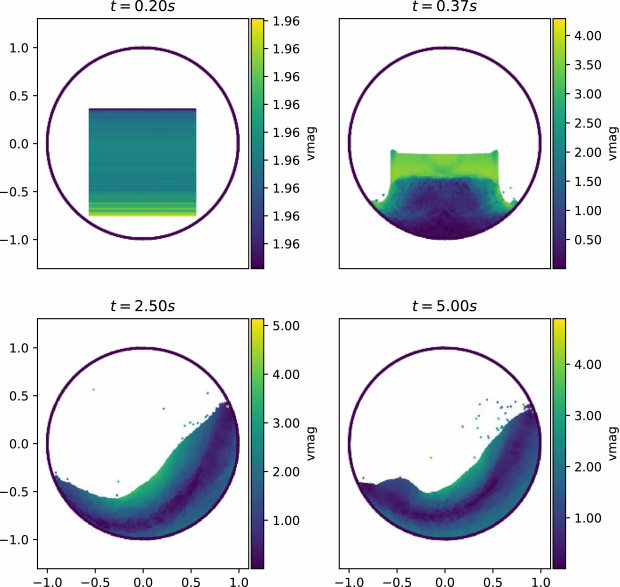
\includegraphics[width=0.6\textwidth]{images/implementation_detail/images/many_bodies/dem_rolling_drum_case}
  \caption{Positions of the sand in a drum, color indicates the velocity magnitude. The top row depicts the
results when the drum is not rotating, and the bottom row is when the drum is rotating.}
\label{fig:dem_drum}
\end{figure}


\FloatBarrier%
\section{Sub-stepping Update Algorithm}
\label{sec:substepping-algorithm}
Problems involving two different materials, such as fluid-structure interaction,
rigid-fluid coupling, etc., involve solving two different materials, such that
one material is stiffer than the other. Let us consider a problem that has both
fluid and solid particles. Assume timesteps of fluid and solid are related as
follows,
\begin{equation}
\Delta t_f = K \Delta t_s,
\end{equation}
where $K$ is some integer. We use a sub-stepping integration scheme to update
the state of \texttt{fluid} and \texttt{solid} particles. Let us say
\texttt{fluid} has $10,000$ particles, and the solid has $1000$ particles, and
let $K$ be $10$. Using a sub-stepping scheme, instead of iterating $10,000$
particles $10$ times, we only do it one time. We first move the higher timestep
material to the next timestep, here fluid, then update the material with lower
timestep $K$ times, such that the simulation is stable.
\begin{figure}[!htpb]
  \centering
  \includegraphics[width=1.0\textwidth]{images/implementation_detail/images/multiphase/time_stepping}
  \caption{Pictorial representation of the sub-stepping algorithm.}
\label{fig:id:multiphase}
\end{figure}
\Cref{fig:id:multiphase} depicts idea of sub-stepping algorithm. Here,
$\Delta t_{\text{factor}}$ is chosen as a timestep for \texttt{solid} particles.
$\Delta t_{\text{factor}}$ is computed based on two factors. One is it is a
integer multiple of $\Delta t_{\text{material 1}}$
(\cref{eqn:id:dt_factor_chose}) and the second is it has to be less than or
equal to $\Delta t_{\text{material 2}}$, such that the simulation is stable.
\begin{equation}
\label{eqn:id:dt_factor_chose}
\Delta t_{\text{factor}} = \frac{\Delta t_{\text{material 1}}}{K}
\end{equation}


\FloatBarrier%
\subsection{Implementation in PySPH}
\label{sec:pysph-substepping-algorithm}
The following integrator routine is used for the sub-stepping algorithm
\lstset{caption={Code snippet for integrator used in substepping.}}
\lstset{basicstyle=\footnotesize\ttfamily}
\begin{lstlisting}[label={contact:equations},frame=lines,language=Python,upquote=True]
class SubSteppingIntegrator(Integrator):
    def one_timestep(self, t, dt):
        self.compute_accelerations()
\end{lstlisting}
We can see that only one method \texttt{self.compute\_accelerations()} is
called at every timestep in a sub-stepping scheme. We use the PySPH feature of
being able to iterate a group of equations to implement this algorithm. We
iterate using the larger $\Delta t$ value, but inside that, we use an iterated
loop with the smaller timestep. The code listing of updating the particle
arrays with different timesteps is given as,
\lstset{caption={Code snippet for substepping algorithm in PySPH.}}
\lstset{basicstyle=\footnotesize\ttfamily}
\begin{lstlisting}[label={contact:equations},frame=lines,language=Python,upquote=True]
  Group(equations=[
      FluidEquations(dest='fluid', sources=['fluid', 'solid'],
                     dt=dt_1)
  ]),
  Group(equations=[
      Group(equations=[
          SolidEquations(dest='solid', sources=['fluid', 'solid'],
                         dt=dt_1/10)
      ])
  ]
  iterate=True, max_iterations=10, min_iterations=10)
\end{lstlisting}
Since here, \texttt{fluid} has a higher timestep, we first update it to the next
timestep using \texttt{FluidEquations} and the \texttt{solid} state is updated
to $t + \Delta t_1$ timestep using $10$ updates with a timestep of
$\frac{\Delta t_1}{10}$. At each iteration we advance the $solid$ particles by
$\Delta t_1 / 10$ time using \texttt{SolidEquations} equations.


\FloatBarrier%
\section{Summary}
\label{sec:id:summary}
In the current chapter, we demonstrated the implementation details of the
algorithms developed in \cref{chap:ctvf,chap:csph}. The PySPH documentation has
implementation details of several algorithms implemented in the above chapters.
We discussed algorithms corresponding to the contact force interaction and
simulation involving two different materials with different timestep values.

A strided array approach is used to track the pairwise contacts. A fixed index
is assigned to the particle for each pairwise interaction with a few bodies
handled. In cases with many bodies, a similar strided approach is used. However,
the contacts are updated dynamically as the particles make and leave contacts.
\Cref{sec:contact-algorithm} utilizes the algorithm of contact tracking for
fewer bodies, while \cref{sec:dem-drum-case} follows the contact tracking
algorithm for many bodies.

A sub-stepping algorithm is discussed in which the material with a higher
timestep is updated first, then the stiffer phase is updated with a lower time
step but in $K$ intervals. We discussed the tools provided by PySPH in order to
implement the sub-stepping algorithm.

In the next chapter, we model the interaction between the fluid and the elastic
structure, fluid-structure interaction. We propose an updated Lagrangian model
by coupling the solver developed in \cref{chap:ctvf} to handle the
fluid-structure interaction problems.
